% Nome do capítulo
\chapter{DESENVOLVIMENTO}
% Label para referenciar
\label{cap4}

% Diminuir espaçamento entre título e texto
\vspace{-1.9cm}

% Texto do capítulo

Este capítulo apresenta as etapas do desenvolvimento do aplicativo.

    \section{Estrutura do Banco de Dados}
    
    \begin{figure}[h]
    \caption{Estrutura do Banco de Dados}
    \centering % para centralizarmos a figura
    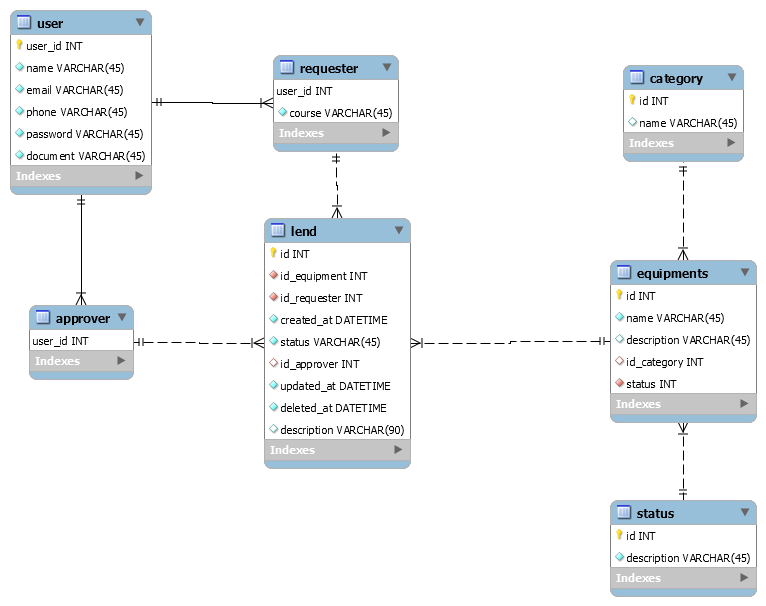
\includegraphics[width=14cm]{imagem/bd-structure.png}
    \caption*{Fonte: Autor}
    \label{figure:bd-structure}
    \end{figure}
    
    \clearpage
    
    As tabelas "requester" e "approver" representam respectivamente usuários do tipo aluno e monitores/técnicos do laboratório e herdam todos os atributos da tabela "user" que representa em si o usuário do sistema. Na tabela "equipments" tem se a relação com a tabela "category" que indica a categoria em que o equipamento está vinculado, enquanto a tabela "status" descreve a disponibilidade no momento de tal equipamento.
    
    A tabela "lend" possui relação com a tabela "requester", "approver" e "equipments", sendo essa entidade responsável por representar as solicitações de empréstimo feitas por alunos, aprovadas ou reprovadas por monitores e/ou técnicos em relação a um equipamento específico que esteja disponível.
    
    \section{Criação da Interface}
    
    A figura \ref{figure:initial-screen} apresenta a tela inicial do aplicativo em seguida a tela de login, na qual os usuários podem realizar o login para ter acesso a tela principal, recuperar a senha, caso necessário e acessar a tela de cadastro para se registrarem no sistema.
    
    \begin{figure}[tb]
    \begin{center}
    \caption{Tela inicial e login}
    
\includegraphics[width=6cm]{imagem/splash-screen.jpg}
    \label{figure:initial-screen}
    \quad
    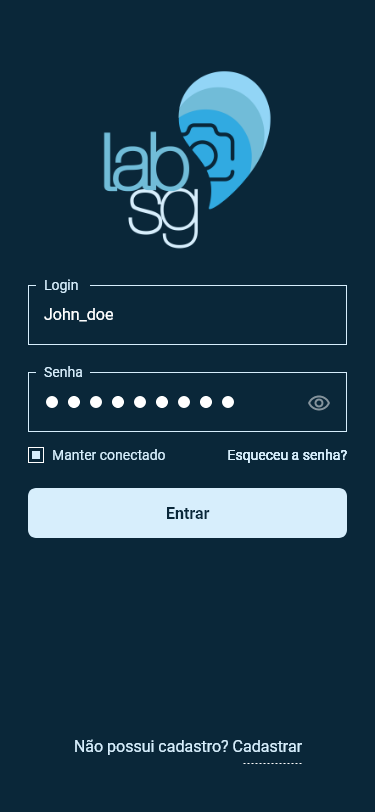
\includegraphics[width=6cm]{imagem/Sign in-1.png}
    \caption*{Fonte: Autor}
    \label{figure:sign-in-screen}
    \end{center}
    \end{figure}
    
    \clearpage
    
    \subsection{Alunos}
    
    Para logar no aplicativo é necessário somente informar o usuário e senha e será redirecionado para a tela principal, na visão do aluno ou na visão de administrador. Ao efetuar o login como aluno, será direcionado a tela representada pela figura \ref{figure:home-solicitante-screen}, cujo alunos poderão pesquisar por equipamentos e verificar a disponibilidade dos mesmos.
    
    \begin{figure}[h]
    \caption{Tela principal do aluno}
    \centering % para centralizarmos a figura
    
\includegraphics[width=6cm]{imagem/Home - Solicitante.png}
    \caption*{Fonte: Autor}
    \label{figure:home-solicitante-screen}
    \end{figure}
    
    Feito a busca pelo equipamento, o aluno pode selecioná lo e preencher as informações adicionais, conforme demonstrado na figura \ref{figure:solicitante} e em seguida solicitar o empréstimo, caso a solicitação seja aprovada e/ou reprovada por algum técnico ou monitor do laboratório, a aplicação emitirá uma notificação para o dispositivo do aluno avisando o sobre a alteração no status da solicitação.
    
    \begin{figure}[tb]
    \begin{center}
    \caption{Busca por equipamento e preenchimento da solicitação}
    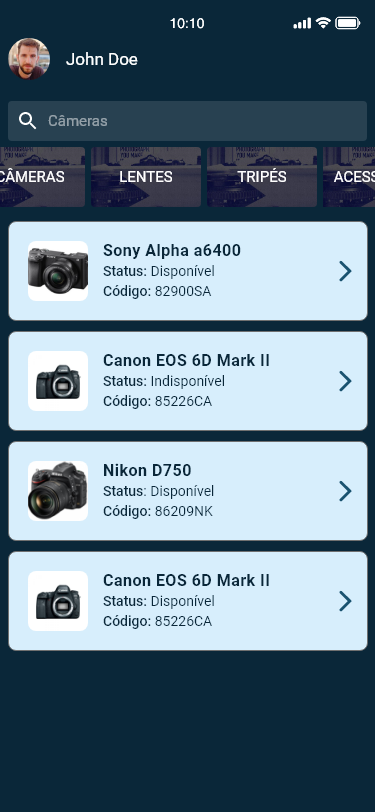
\includegraphics[width=6cm]{imagem/Solicitante on search.png} \quad
    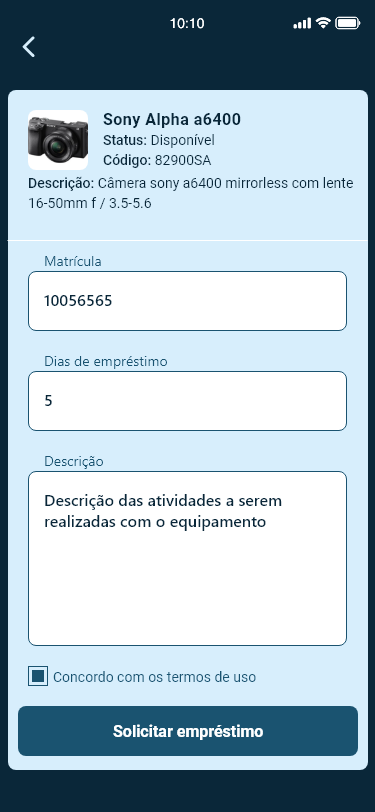
\includegraphics[width=6cm]{imagem/Solicitante on loan.png}
    \caption*{Fonte: Autor}
    \label{figure:solicitante}
    \end{center}
    \end{figure}
    
    Caso a solicitação seja aprovada, o aluno receberá uma notificação avisando o sobre o prazo de devolução do equipamento, seguindo o número de dias preenchido na solicitação do equipamento.
    
    \clearpage
    
    \subsection{Monitores e técnicos}
    
    Ao efetuar o login como monitor ou técnico, será direcionado a tela representada pela figura \ref{figure:home-aprovador-screen} e poderá ter acesso a consulta de equipamentos cadastrados, solicitações de empréstimos pendentes e ao cadastro de novos equipamentos, se necessário.
    
    \begin{figure}[h]
    \caption{Tela principal de monitores e técnicos}
    \centering % para centralizarmos a figura
    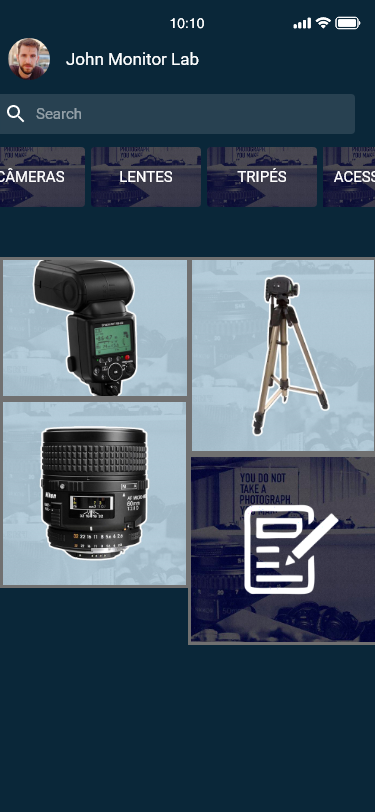
\includegraphics[width=6cm]{imagem/Home - Aprovador.png}
    \caption*{Fonte: Autor}
    \label{figure:home-aprovador-screen}
    \end{figure}
    
    O processo de cadastro de equipamentos inicia com a interação entre algumas das imagens presentes na tela principal dos tipos de equipamentos que podem ser cadastrados na plataforma. Após interagir com algum dos componentes que possuem essa funcionalidade, o usuário é redirecionado para a tela de cadastro e poderá fazer o upload de uma imagem do equipamento, além de preencher as informações sobre o mesmo para cadastrar.
    
    \clearpage
    
    \begin{figure}[tb]
    \begin{center}
    \caption{Cadastro de novos equipamentos}
    \includegraphics[width=6cm]{imagem/Home - Aprovador – add new equip.png} \quad
    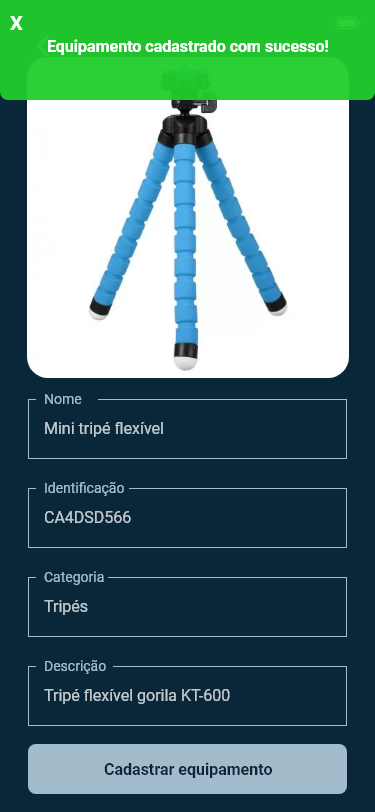
\includegraphics[width=6cm]{imagem/Home - Aprovador – add new equip – 1.png}
    \caption*{Fonte: Autor}
    \label{figure:aprovador-equip}
    \end{center}
    \end{figure}
    
    O aplicativo também possibilita que monitores e técnicos verifiquem solicitações de empréstimos feitas por alunos e aprovam/reprovam as de acordo com a figura \ref{figure:aprovador-solic}, após essa ação o aluno solicitante recebe uma notificação informando se sua solicitação foi aprovada ou reprovada.
    
    \clearpage
    
    \begin{figure}[tb]
    \begin{center}
    \caption{Busca por solicitações e aprovação/reprovação}
    \includegraphics[width=6cm]{imagem/Home - Aprovador – list lends.png} \quad
    \includegraphics[width=6cm]{imagem/Home - Aprovador – approve lends.png}
    \caption*{Fonte: Autor}
    \label{figure:aprovador-solic}
    \end{center}
    \end{figure}

    
    